%------------------------------------------------
\section{Overview of problem}
%------------------------------------------------
\begin{frame}[t]
	\frametitle{COVID-19 incidence forecasting}
	\tikzstyle{background grid}=[draw, black!50,step=.5cm]
	%
	How to \emph{design} a machine learning model for forecasting a time-series?\\
	%
	\tikzstyle{background grid}=[draw, black!50,step=.5cm]
	\begin{tikzpicture}[remember picture, overlay] %show background grid, 
		% Put the graphic inside a node. This makes it easy to place the
		% graphic and to draw on top of it. 
		% The above right option is used to place the lower left corner
		% of the image at the (0,0) coordinate. 
		\node [inner sep=0pt,above right, opacity=1.0]  at (0.0\textwidth,-0.72\textheight) (raw data) 
			{
				\only<1>{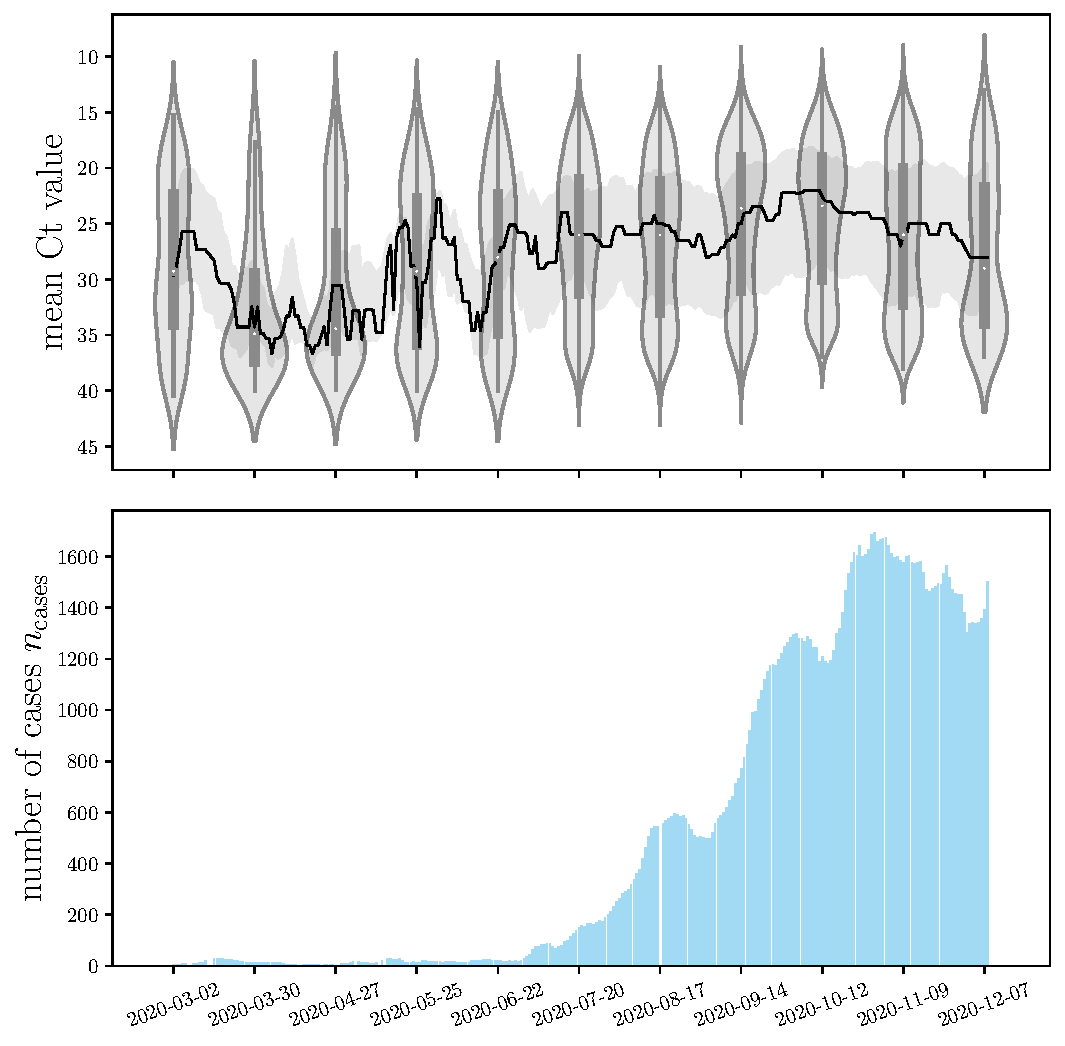
\includegraphics[width=0.43\textwidth]{raw_data/animation_0.pdf}}%
				\only<2>{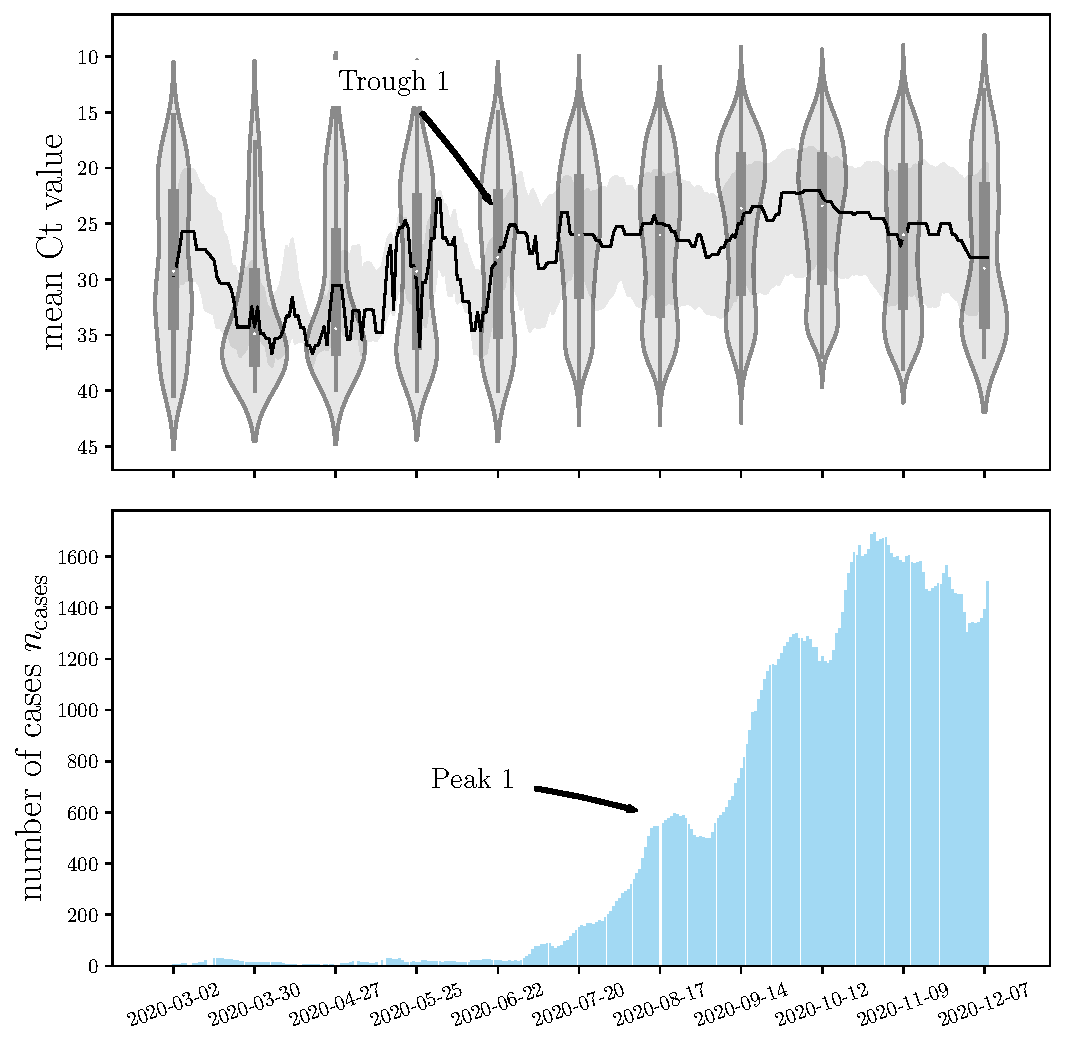
\includegraphics[width=0.43\textwidth]{raw_data/animation_1.pdf}}%
				\only<3>{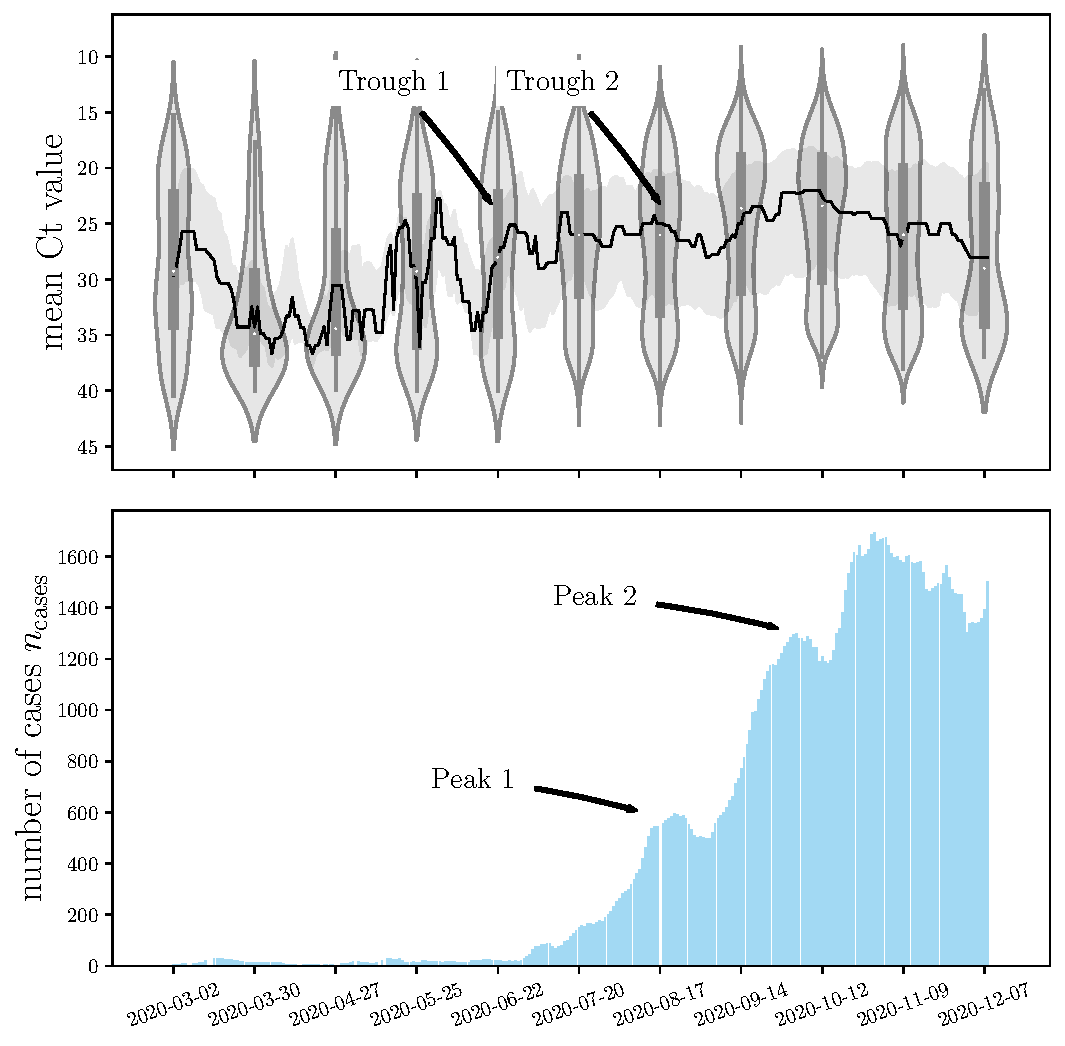
\includegraphics[width=0.43\textwidth]{raw_data/animation_2.pdf}}%
				\only<4->{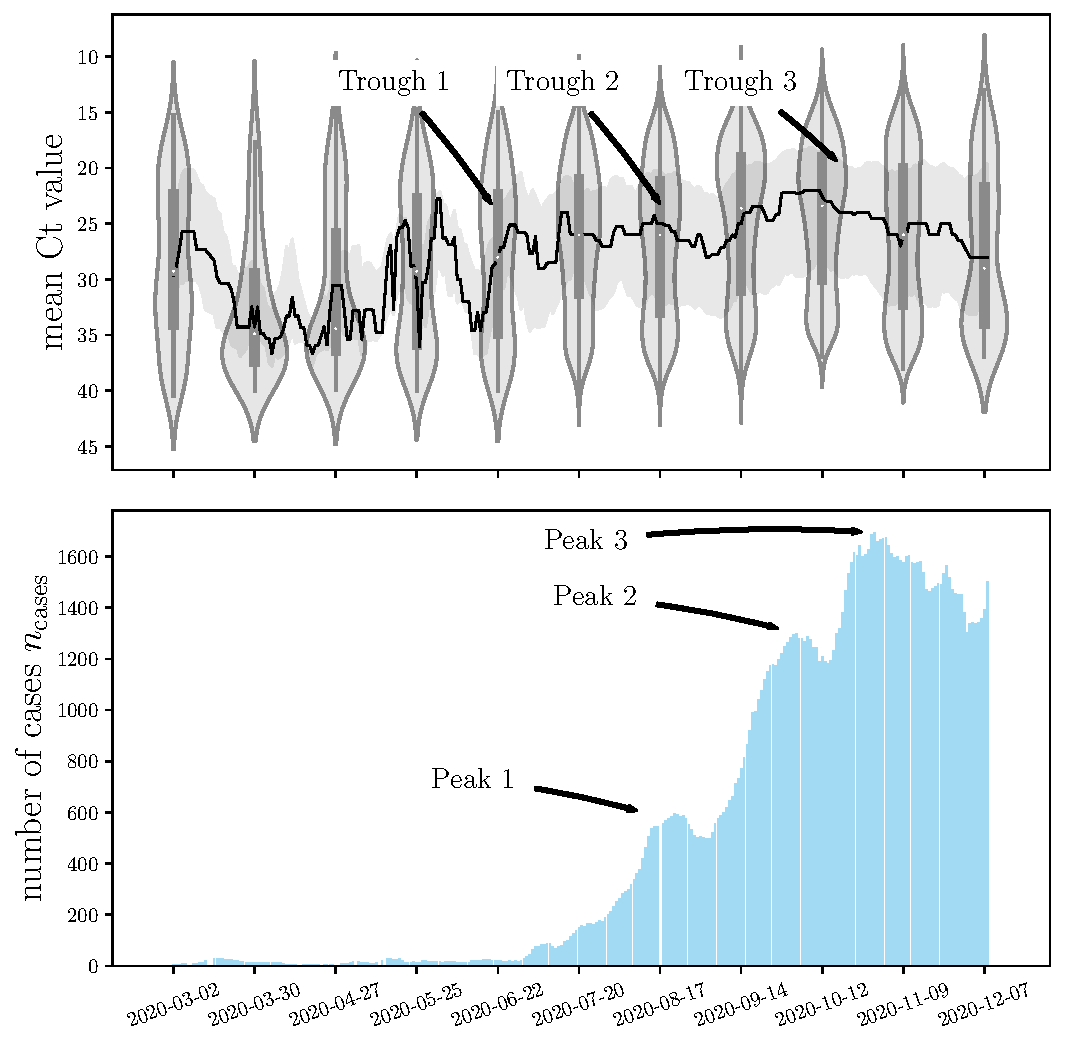
\includegraphics[width=0.43\textwidth]{raw_data/animation_3.pdf}}%
			};
		\node [inner sep=0pt,above left, opacity=1.0]  at (0.99\textwidth,-0.65\textheight) (seq2seq) 
			{
				\only<5>{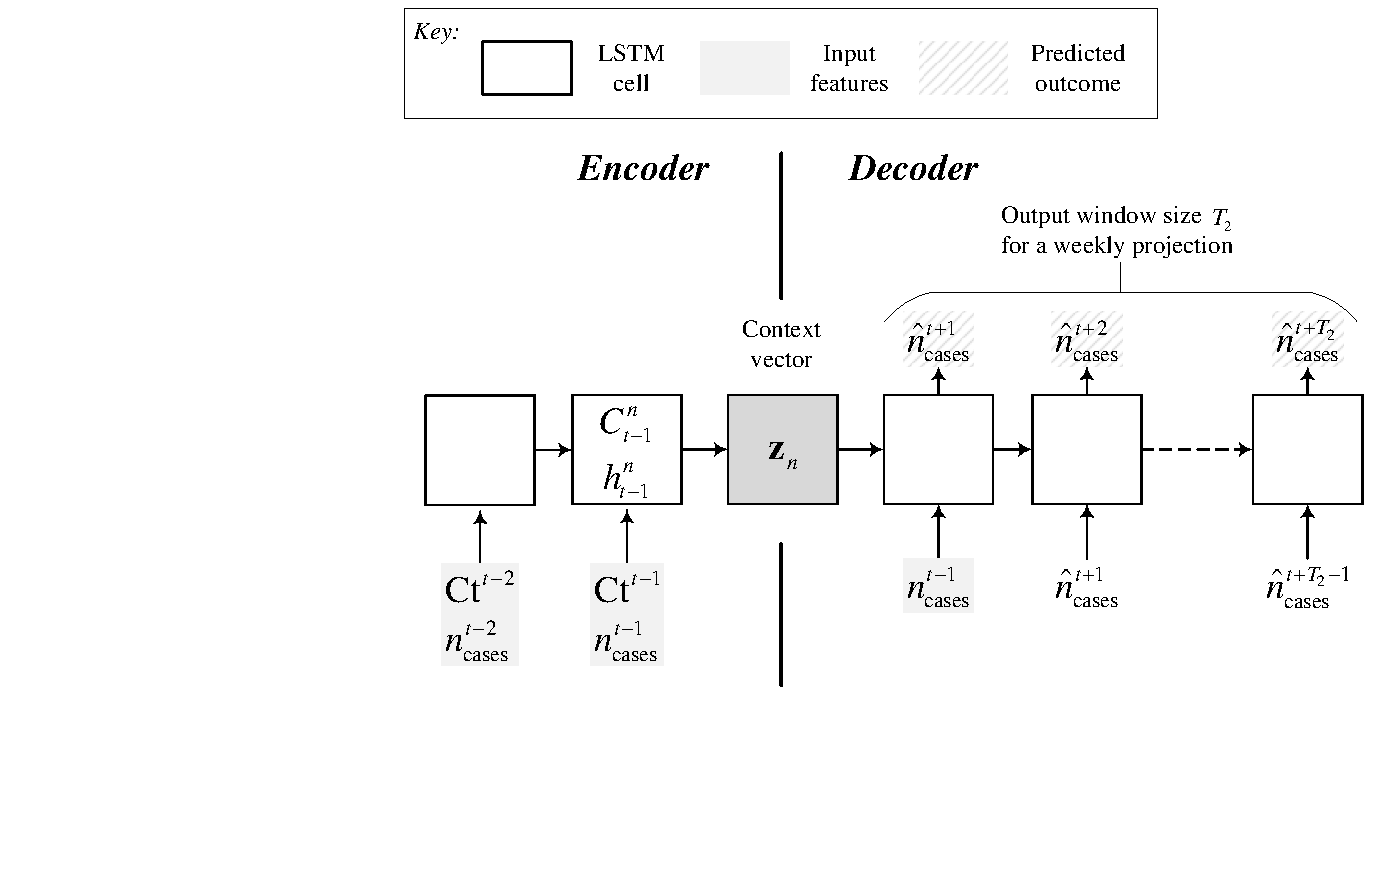
\includegraphics[width=0.55\textwidth]{model_1.pdf}}%
				\only<6>{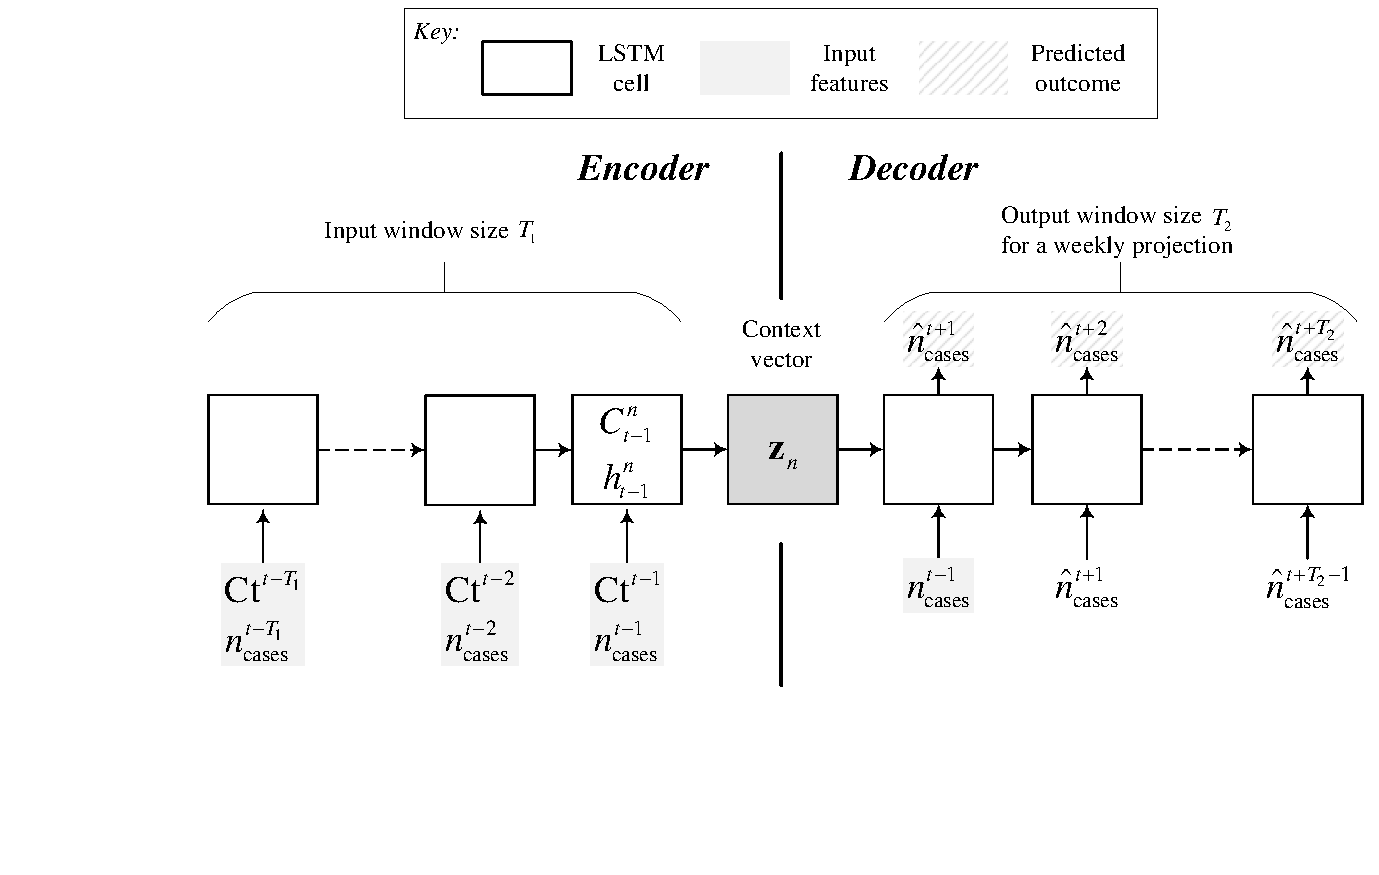
\includegraphics[width=0.55\textwidth]{model_2.pdf}}%
				\only<7>{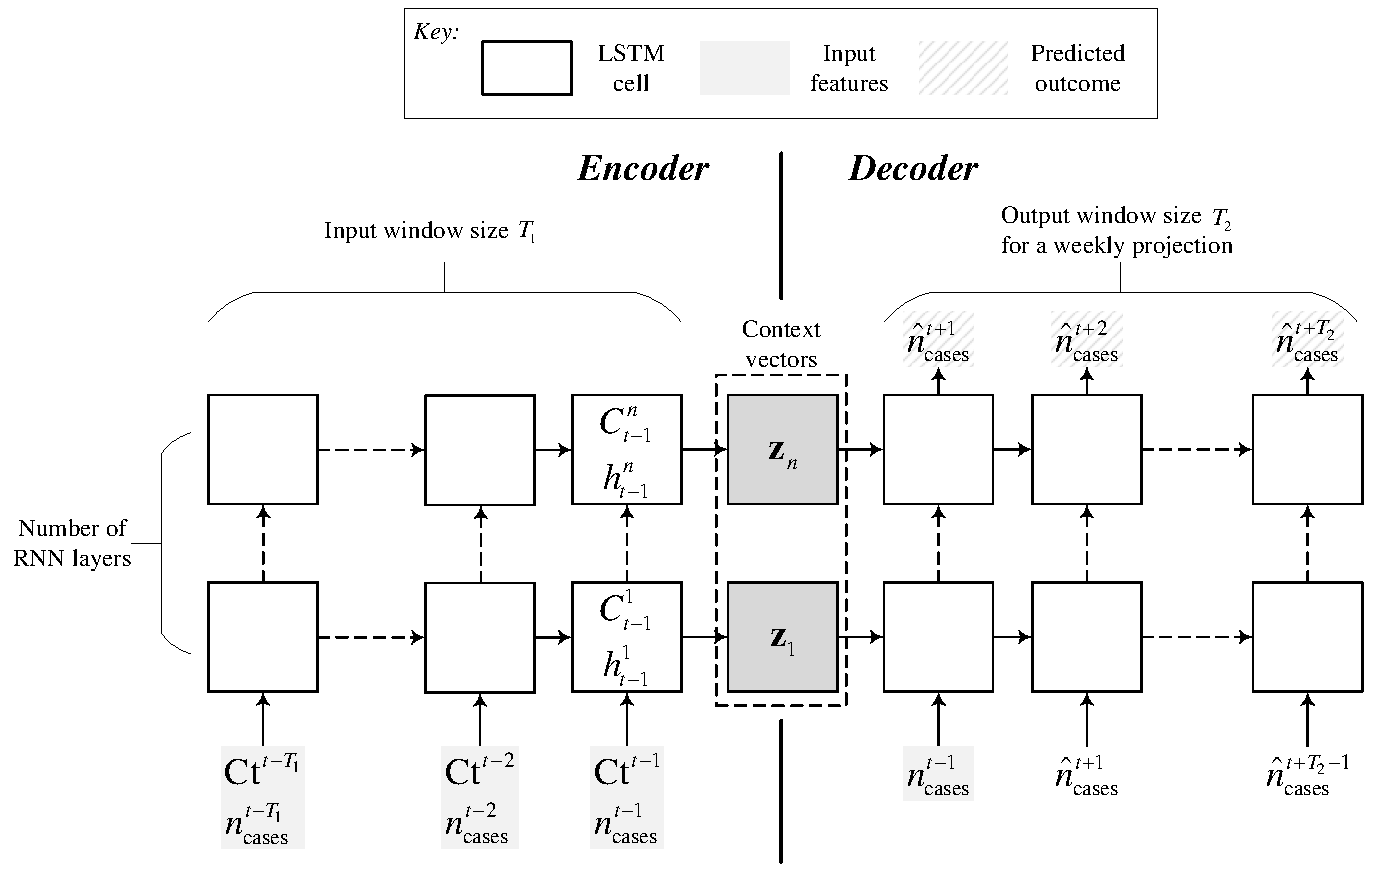
\includegraphics[width=0.55\textwidth]{model_3.pdf}}%
			};
		\only<5->{
			\node[inner sep=0pt,below=\belowcaptionskip of seq2seq,text width=\linewidth]
				{\vspace{-1em}{Seq2Seq model}};
		}%
		\node [inner sep=0pt, opacity=1.0]  at (0.43\textwidth,-0.15\textheight) (ct) {};%
		\node [inner sep=0pt, opacity=1.0]  at (0.43\textwidth,-0.50\textheight) (cases) {};%
		\only<-6>{
			\node [inner sep=0pt, opacity=1.0]  at (0.65\textwidth,-0.50\textheight) (input) {};%
		}%
		\only<7->{
			\node [inner sep=0pt, opacity=1.0]  at (0.60\textwidth,-0.60\textheight) (input) {};%
		}%
		% show origin
		% \fill (0,0) circle (2pt);
	\end{tikzpicture}%
	%
	\begin{tikzpicture}[overlay]
		\only<5->{\path[->,magenta,thick] (ct) edge [out=0, in=270] (input);}
		\only<5->{\path[->,magenta,thick] (cases) edge [out=0, in=270] (input);}
	\end{tikzpicture}%
	%
	\vspace{-3em}
\end{frame}
